\documentclass[apjl]{emulateapj}
%\documentclass[letterpaper,12pt,preprint]{aastex}

% packages
\usepackage{amssymb,amsmath,amsbsy}
\usepackage{booktabs}
\usepackage{multirow}
\usepackage{url}

% commands
\newcommand{\given}{\,|\,}
\newcommand{\dd}{\mathrm{d}}
\newcommand{\transpose}[1]{{#1}^{\mathsf{T}}}
\newcommand{\inverse}[1]{{#1}^{-1}}
\newcommand{\Msun}{\ifmmode {{\rm M}_{\odot}}\else M$_{\odot}$\fi}
\newcommand{\bs}[1]{\boldsymbol{#1}}
\newcommand{\degree}{^{\circ}}
\newcommand{\eqn}{Equation~}

% Symbols
\newcommand{\period}{T}
\newcommand{\mf}{m_f}
\newcommand{\wdupper}{1.44}

\begin{document}

\title{The mass distribution of companions to low-mass white dwarfs}
\author{Jeff J. Andrews\altaffilmark{\colum}, Adrian M. Price-Whelan\altaffilmark{\colum}, Marcel Ag\"ueros\altaffilmark{\colum}}

% Affiliations
\newcommand{\colum}{1}
\altaffiltext{\colum}{Department of Astronomy, 
		              Columbia University, 
		              550 W 120th St., 
		              New York, NY 10027, USA}


\begin{abstract}
Measuring the masses of companions to single-line spectroscopic binary stars
is (in general) not possible because of the unknown orbital plane inclination angles. 
Even when the mass of the visible star can be measured, only a lower limit can be placed
on the mass of the unseen companion. However, since these inclination angles should be isotropically
distributed, for a large enough, unbiased sample, the 
companion mass distribution can be deconvolved from the distributions of observables.
In this work, we construct a hierarchical probabilistic model to infer properties of unseen 
companion stars to low mass white dwarfs (LMWD) given orbital period and projected radial velocity measurements of the primary. We use a mixture of 
two Gaussians to model the true companion mass distribution to represent 
populations of white dwarfs (WD) and neutron stars (NS). 
Our model successfully recovers the initial parameters of several mock data sets.
We then apply our model to 55 of the 61 white dwarfs in 
the extremely low mass (ELM) WD survey. We find maximum a posteriori parameters for
the WD companion population of $\mu_{\rm WD} = 0.71~\Msun$ and $\sigma_{\rm WD} = 0.26~\Msun$ 
with a NS fraction consistent with zero, $f_{\rm NS} = 0\%$. However, the marginal posterior 
distribution over NS fraction has a significant tail up to $f_{\rm NS} \approx 16\%$.
We make samples from the posterior distribution publicly available so that future observational
efforts may compute the NS probability for newly discovered low mass WDs.
\end{abstract}

\keywords{binaries: general --- binaries: spectroscopic --- methods: statistical --- white dwarfs} 

\section{Introduction}

Except in special cases of extreme metallicity \citep{kilic07}, the Galaxy is not old enough to produce LMWDs ($M\lesssim0.45~ \Msun$) through single star evolution. These objects are formed through dynamical interactions with another star, and are therefore expected to be found in binary systems \citep{han98,nelemans00,nelemans01,vdSluys06,woods12}. In their seminal work, \citet{marsh95} discovered companions around five LMWDs in their sample of seven objects, confirming these theoretical expectations. The ELM WD Survey identifies LMWDs in SDSS and elsewhere for spectroscopic follow-up, focusing in particular on extremely low mass WDs ($M\lesssim0.3~ \Msun$) \citep{ELMI}. After their initial investigation found 11 of 12 LMWDs had close binary companions, further spectroscopic follow-up has now brought the sample of ELM WDs to 61 systems, 55 of which have measured radial velocity amplitudes and orbital periods; we refer to this as the ELM sample \citep{ELMII, ELMIII, ELMIV, ELMV}.


While the orbital periods and radial velocities indicated the companions were most likely WDs, due to the unmeasured inclination angle, these LMWDs could host NS companions \citep{vLeeuwen07}. Indeed, LMWDs are observed as companions of millisecond pulsars \citep{vKerkwijk96,callanan98,bassa06,antoniadis12}. However, all radio searches for pulsed emission, as well as searches for blackbody X-ray emission from a NS surface have been unsuccessful \citep{agueros09a,agueros09b,kilic13}. 

%Such systems are extremely interesting: the NS binaries with WD companions bright enough to detect spectroscopic radial velocity variations have precisely determined NS masses which provide useful insights into the binary evolution processes that form these systems \citep{benvenuto05,smedley14,jia14}.


%Selecting the most likely candidates for multiwavelength follow-up is crucial.

Spectroscopic fits determine which systems are ideal candidates for spectroscopic follow-up; for each LMWD in the ELM sample, spectroscopic observations provide the orbital period ($\period$), primary WD mass ($M_1$), and projected orbital velocity ($K=v \sin i$). Using Kepler's third law, we can write the relation between these quantities and the unknown inclination angle as:
\begin{equation}
	\frac{(M_2 \sin i)^3}{\left(M_1+M_2\right)^2} = \frac{\period}{2\pi G} K^3 = \mf \label{eq:massfunc}
\end{equation}
The righthand side of this equation is the mass function ($\mf$). $M_2$ is minimized for an edge-on orbit, with $i = 90\degree$. Because of the dependence on $i$, the nature of the companion cannot usually be determined based on $\mf$ alone. Figure~\ref{fig:Porb-M1} shows that the population of LMWD with pulsar companions (triangles) occupy the same region in $M_1 - \period$ space as those with WD companions (circles). Therefore, barring rare circumstances (such as an edge-on, eclipsing system), individual LMWDs with NS companions cannot be readily identified.


The ELM sample is now large enough that the companion mass distribution, and importantly the NS fraction can be statistically constrained. In this work, we develop a probabilistic model to infer parameters of an assumed form for the mass distribution of companions to ELM WDs. Our method is similar to that employed by \citet{ozel12} and \citet{kiziltan13} to describe the mass distribution of NSs in binaries using post-Keplerian parameters. We focus on several specific astrophysical questions: 1.\ Can the population as a whole be modeled using a simple description of the companion masses? 2.\ How does the companion mass distribution compare to predictions from population synthesis simulations?  3.\ What is the rate of NS-LMWD binaries implied by our model? 4.\ What are the resulting distributions of NS probabilities for individual systems in the ELM sample? 


To answer these questions, we build the mathematical framework in Section 2, then apply our model to test and real data in Section 3. We give the results and discussion in Section 4, and conclude in Section 5.

\begin{figure}[h!]
\begin{center}
\includegraphics[angle=90,width=0.95\columnwidth]{Porb_M1.eps}
\caption{The $\period$ - $M_1$ distribution of the ELM WD sample (circles) and the known WD-NS binaries (triangles). The three eclipsing systems in the ELM sample with known $M_2$ are shown as filled circles, and the ELM WDs without detected radial velocity variations are shown by the arrows. From $\period$ and $M_1$ alone, the two populations are indistinguishable.}
\label{fig:Porb-M1}
\end{center}
\end{figure}




\section{Methods}

We construct a statistical model to derive constraints on a parametric model for the distribution of ELM WD companion masses, $p(M_2 \given \bs{\theta})$.\footnote{In what follows, vectors or sets of parameters or quantities are represented by bold symbols.} For each system, we assume we are given $K$, $T$, and $M_1$ and therefore know the value of the mass function, $\mf$ (\eqn~\ref{eq:massfunc}). We would like to derive posterior constraints on the parameters, $\bs{\theta}$, that describe the distribution of companion masses, $p(M_2\given \bs{\theta})$, given all of the observed mass functions, $\bs{m}_f$, by deconvolving the distribution of mass functions from the unobserved inclination angle, $i$. Using Bayes' rule,
\begin{equation}
    p(\bs{\theta} \given \bs{\mf}) = \frac{1}{\mathcal{Z}}~p(\bs{\mf} \given \bs{\theta})~p(\bs{\theta}).
\end{equation}
where $p(\bs{\mf} \given \bs{\theta})$ is the likelihood, $p(\bs{\theta})$ is the prior on parameters $\bs{\theta}$, and the evidence integral, $\mathcal{Z}$, is a constant that depends only on the data. The likelihood, $p(\bs{\mf} \given \bs{\theta})$, can be split into a product over the likelihoods of individual systems:

\begin{equation}
p(\bs{\mf} \given \bs{\theta}) = \prod_j p(\mf \given \bs{\theta})
\end{equation}

where the product is over each of the $j$ systems.  This marginal likelihood involves integrals over the latent variables $i$ and $M_2$,
\begin{align}
    p(\mf \given \bs{\theta}) &= \int_{-\infty}^\infty dM_2 \int_0^{\pi/2} di  \nonumber \\
      & \qquad {} \times p(\mf \given M_1, M_2, i)~p(M_2 \given \bs{\theta})~p(i).
\end{align}
We neglect observational uncertainties in $\mf$ and $M_1$,\footnote{The fractional uncertainties in these quantities are small, $\sigma_x / x \sim 0.05-0.1$.} and assume the inclination angles are isotropically distributed
\begin{equation}
	p(\mf \given M_1, M_2, i) = \delta \left[\mf - f(M_1, M_2, i) \right]
\end{equation}
where
\begin{equation}
	f(M_1, M_2, i) = \frac{(M_2 \sin i)^3}{(M_1 + M_2)^2}
\end{equation}
and
\begin{equation}
	p(i) = \sin i.
\end{equation}
For now, we do not specify a parametric form for the companion mass distribution, $p(M_2 \given \bs{\theta})$. With the above assumptions, the marginal likelihood integral is
\begin{align}
%    p(\mf \given \bs{\theta}) &= \int_{0}^\infty dM_2~p(M_2 \given \bs{\theta}) \int_0^{\pi/2} di \nonumber \\
%    & \qquad {} \times \delta \left[\mf - f(M_1, M_2, i)\right]~\sin i\\
    p(\mf \given \bs{\theta}) &= \int_{0}^\infty dM_2 ~p(M_2 \given \bs{\theta})  \nonumber \\
    & \qquad {} \times \int_0^{\pi/2} di ~\sin i ~ \delta \left[g(M_1,M_2,i) \right]\label{eq:delta}
\end{align}
where
\begin{equation}
	g(M_1,M_2,i) = \mf - \frac{M_2^3}{(M_1+M_2)^2}\sin^3 i.
\end{equation}
The inner integral (over $i$) has the form
\begin{equation}
    \int dx~F(x)~\delta \left[ G(x) \right] = \sum_j \frac{F(x^*_j)}{|G'(x^*_j)|}
\end{equation}
where the sum is over the roots, $x^*_j$, of the function $G(x)$. The root, $i^*$, and derivative of the argument of the delta function in \eqn\ref{eq:delta} are 
\begin{align}
%	\sin i^* &= \alpha\\
%	\alpha &= \frac{(\mf(M_1+M_2)^2)^{1/3}}{M_2}\\
	\sin i^* &= \frac{ \left[\mf(M_1+M_2)^2 \right]^{1/3}}{M_2}\\
%	\frac{\partial g}{\partial i} &= \frac{3M_2^3}{(M_1+M_2)^2}\sin^2 i \cos i\\
%	\frac{\partial g}{\partial i}\bigg\rvert_{i^*} &= \frac{3M_2^3}{(M_1+M_2)^2} \alpha^2 \sqrt{1 - \alpha^2}
	\frac{\partial g}{\partial i}\bigg\rvert_{i^*} &= \frac{3M_2^3}{(M_1+M_2)^2} \sin^2 i^* \sqrt{1 - \sin^2 i^*}
\end{align}
We may rewrite the marginal likelihood as
\begin{align}
	p(\mf \given \bs{\theta}) &= \int_{0}^\infty dM_2~p(M_2 \given \bs{\theta})~\sin i^* \left(\frac{\partial g}{\partial i}\bigg\rvert_{i^*}\right)^{-1}\\
%	&= \int_{0}^\infty dM_2~p(M_2 \given \bs{\theta})~\alpha\left[\frac{3M_2^3}{(M_1+M_2)^2} \alpha^2 \sqrt{1 - \alpha^2}\right]^{-1}\\
	&= \int_{M_{2,{\rm min}}}^\infty dM_2~p(M_2 \given \bs{\theta})~h(M_2, \mf, M_1) \label{eq:fullm2}
\end{align}

where the bottom bound in the integral in \eqn\ref{eq:fullm2} is set by the minimum companion mass for which the integrand is real, $M_{2,{\rm min}}$ (determined by setting $i=90\degree$ in \eqn\ref{eq:massfunc} and solving for $M_2$), and

\begin{equation}
h(M_2, \mf, M_1) = \frac{(M_1+M_2)^{4/3}}{3\ \mf^{1/3}M_2\sqrt{M_2^2 - \left[ \mf(M_1+M_2)^2 \right]^{2/3}}}
\end{equation}


\subsection{Our Model} \label{sec:experiments}

We must now choose a functional form for the companion mass distribution,  $p(M_2\given \bs{\theta})$. For all experiments -- including that with the real data -- we use a two component Gaussian mixture model to fit the data. In tests below, we generate test data with different mixture component forms. We truncate the distributions using physically motivated bounds so that the white dwarf component is restricted to the range $M_2\in (0.2,\wdupper)~\Msun$ and the neutron star component is restricted to the range $M_2\in (1.3,2)~\Msun$,
\begin{align}
%	h(M_2, \mf, M_1) &= \frac{(M_1+M_2)^{4/3}}{3\mf^{1/3}M_2\sqrt{M_2^2 - \left[ \mf(M_1+M_2)^2 \right]^{2/3}}}\\
%	p(\mf \given \bs{\theta}) &= \int_{0}^\infty dM_2~\left[ (1-f_{\rm NS})p_{\rm WD} + f_{\rm NS}p_{\rm NS} \right]~h(M_2, \mf, M_1)\\
	p(M_2 \given \bs{\theta}) &= \left[ (1-f_{\rm NS})~p_{\rm WD} + f_{\rm NS}~p_{\rm NS} \right] 
\end{align}
where 
\begin{align}
	p_{\rm WD} &= \mathcal{N}(M_2 \given \mu_{\rm WD}, \sigma^2_{\rm WD}); ~0.2 < \frac{M_2}{\Msun} < \wdupper \\
	p_{\rm NS} &= \mathcal{N}(M_2 \given \mu_{\rm NS}, \sigma^2_{\rm NS}); ~1.3 < \frac{M_2}{\Msun} < 2.
\end{align}
and $\mathcal{N}$ is the (truncated, but properly normalized) normal distribution with mean $\mu$ and variance $\sigma^2$ and the distributions are limited to the ranges specified. In this work, we fix the mean and variance of the neutron star distribution to
\begin{align}
	\mu_{\rm NS} &= 1.4~\Msun\\
	\sigma^2_{\rm NS} &= (0.05~\Msun)^2
\end{align}
based on indications that NSs in certain binaries may be somewhat more massive than the canonical NS mass of 1.35 \Msun~ \citep{kiziltan13,smedley14}. The probability of any particular system having a NS companion $P_{\rm NS}$ is then:
\begin{equation}
P_{\rm NS} = \int_{0}^{\infty} dM_2~ f_{\rm NS}~ p_{\rm NS}~ h(M_2, \mf, M_1) \label{eq:P_NS}
\end{equation}


Our companion mass model parameters are then $\bs{\theta} = (\mu_{\rm WD}, \sigma_{\rm WD}, f_{\rm NS})$. We choose uninformative priors on these parameters: for the mean of the white dwarf component, we use a uniform distribution from $0.2-1.4~\Msun$; we use a (scale-invariant) logarithmic prior for the variance of the white dwarf component over the range $0.05-2~\Msun$; finally, we use a uniform prior over the dimensionless neutron star fraction from $0-1$. The model parameters are summarized in Table~\ref{tbl:parameters}.

%\setlength{\tabcolsep}{2pt}
\renewcommand{\arraystretch}{1.405}
\begin{deluxetable}{ccccc}
	\tablecaption{Model Results \label{tbl:parameters}}

	\tablehead{
		\multicolumn{2}{c}{} &
		\colhead{$\mu_{\rm WD}$} & 
		\colhead{$\sigma_{\rm WD}$} &
		\colhead{$f_{\rm NS}$} \\
		\colhead{} &
		\colhead{} &
		\colhead{[\Msun]} &
		\colhead{[\Msun]} &
		\colhead{}
	}

	\startdata
		\multicolumn{2}{c}{\multirow{2}{*}{Priors}} & $\mathcal{U}(0.2, 1)$ & $\propto \sigma^{-1}$  & $\mathcal{U}(0, 1)$ \\
		\multicolumn{2}{c}{} & & $(0.02 < \sigma/\Msun < 2)$ & \\
		\cutinhead{Test Cases}
		\multirow{2}{*}{Test 1} & True & 0.7 & 0.2 & 0.0 \\
		 & MAP & 0.74 & 0.18 & 0.0 \\
		 \hline
		\multirow{2}{*}{Test 2} & True & 0.7 & 0.2 & 0.1 \\
		 & MAP & 0.76 & 0.17 & 0.12 \\
		 \hline
		\multirow{2}{*}{Test 3} & True & \nodata & \nodata & 0.1 \\
		 & MAP & 0.80 & 0.39 & 0.12 \\
		 \cutinhead{ELM Sample}
		 & MAP & 0.71 & 0.26 & 0.0
	\enddata

	\tablecomments{Parameter information for the form of the companion mass distribution used in the experiments of Section~\ref{sec:experiments}. $\mathcal{U}$ is the uniform distribution. There are 3 free parameters. We additionally fix the NS distribution: $\mu_{\rm NS} = 1.4~\Msun$ and $\sigma_{\rm NS} = 0.05~\Msun.$}\

\end{deluxetable}


We use an ensemble Markov Chain Monte Carlo algorithm \citep{goodman10} to draw samples from the posterior distribution, $p(\mu_{\rm WD}, \sigma_{\rm WD}, f_{\rm NS} \given \bs{m}_f, \bs{M}_1)$. The algorithm is implemented in the \texttt{Python} programming language \citep[{\tt emcee};][]{foremanmackey13} and uses an ensemble of individual ``walkers'' to naturally adapt to the geometry of the parameter-space being explored. We run the walkers for an initial, burn-in period of 500 steps starting from randomly drawn initial conditions (sampled from the priors in Table~\ref{tbl:parameters}). We then re-initialize the walkers from their positions at the end of this run and run again for 1000 steps. We throw out the burn-in samples to eliminate any effects from our choice of initial conditions. The autocorrelation times for each parameter confirm they have converged.


\section{Applying Our Model} \label{sec:tests}
To test the performance of this Gaussian mixture model, we first apply it to three separate sets of mock data (described in detail below), each with 100 ``observed'' systems. These data are generated by randomly drawing the companion mass, $M_2$, from a particular distribution, then using a randomly drawn inclination angle and primary mass, $M_1$, to compute the mass function, $\mf$. We draw $M_1$ from a uniform distribution, $\mathcal{U}(0.2,0.4)~\Msun$. We apply the same Gaussian mixture model to all test datasets to infer the parameters of the white dwarf mixture component and neutron star fraction.


\begin{figure*}[h!]
\begin{center}
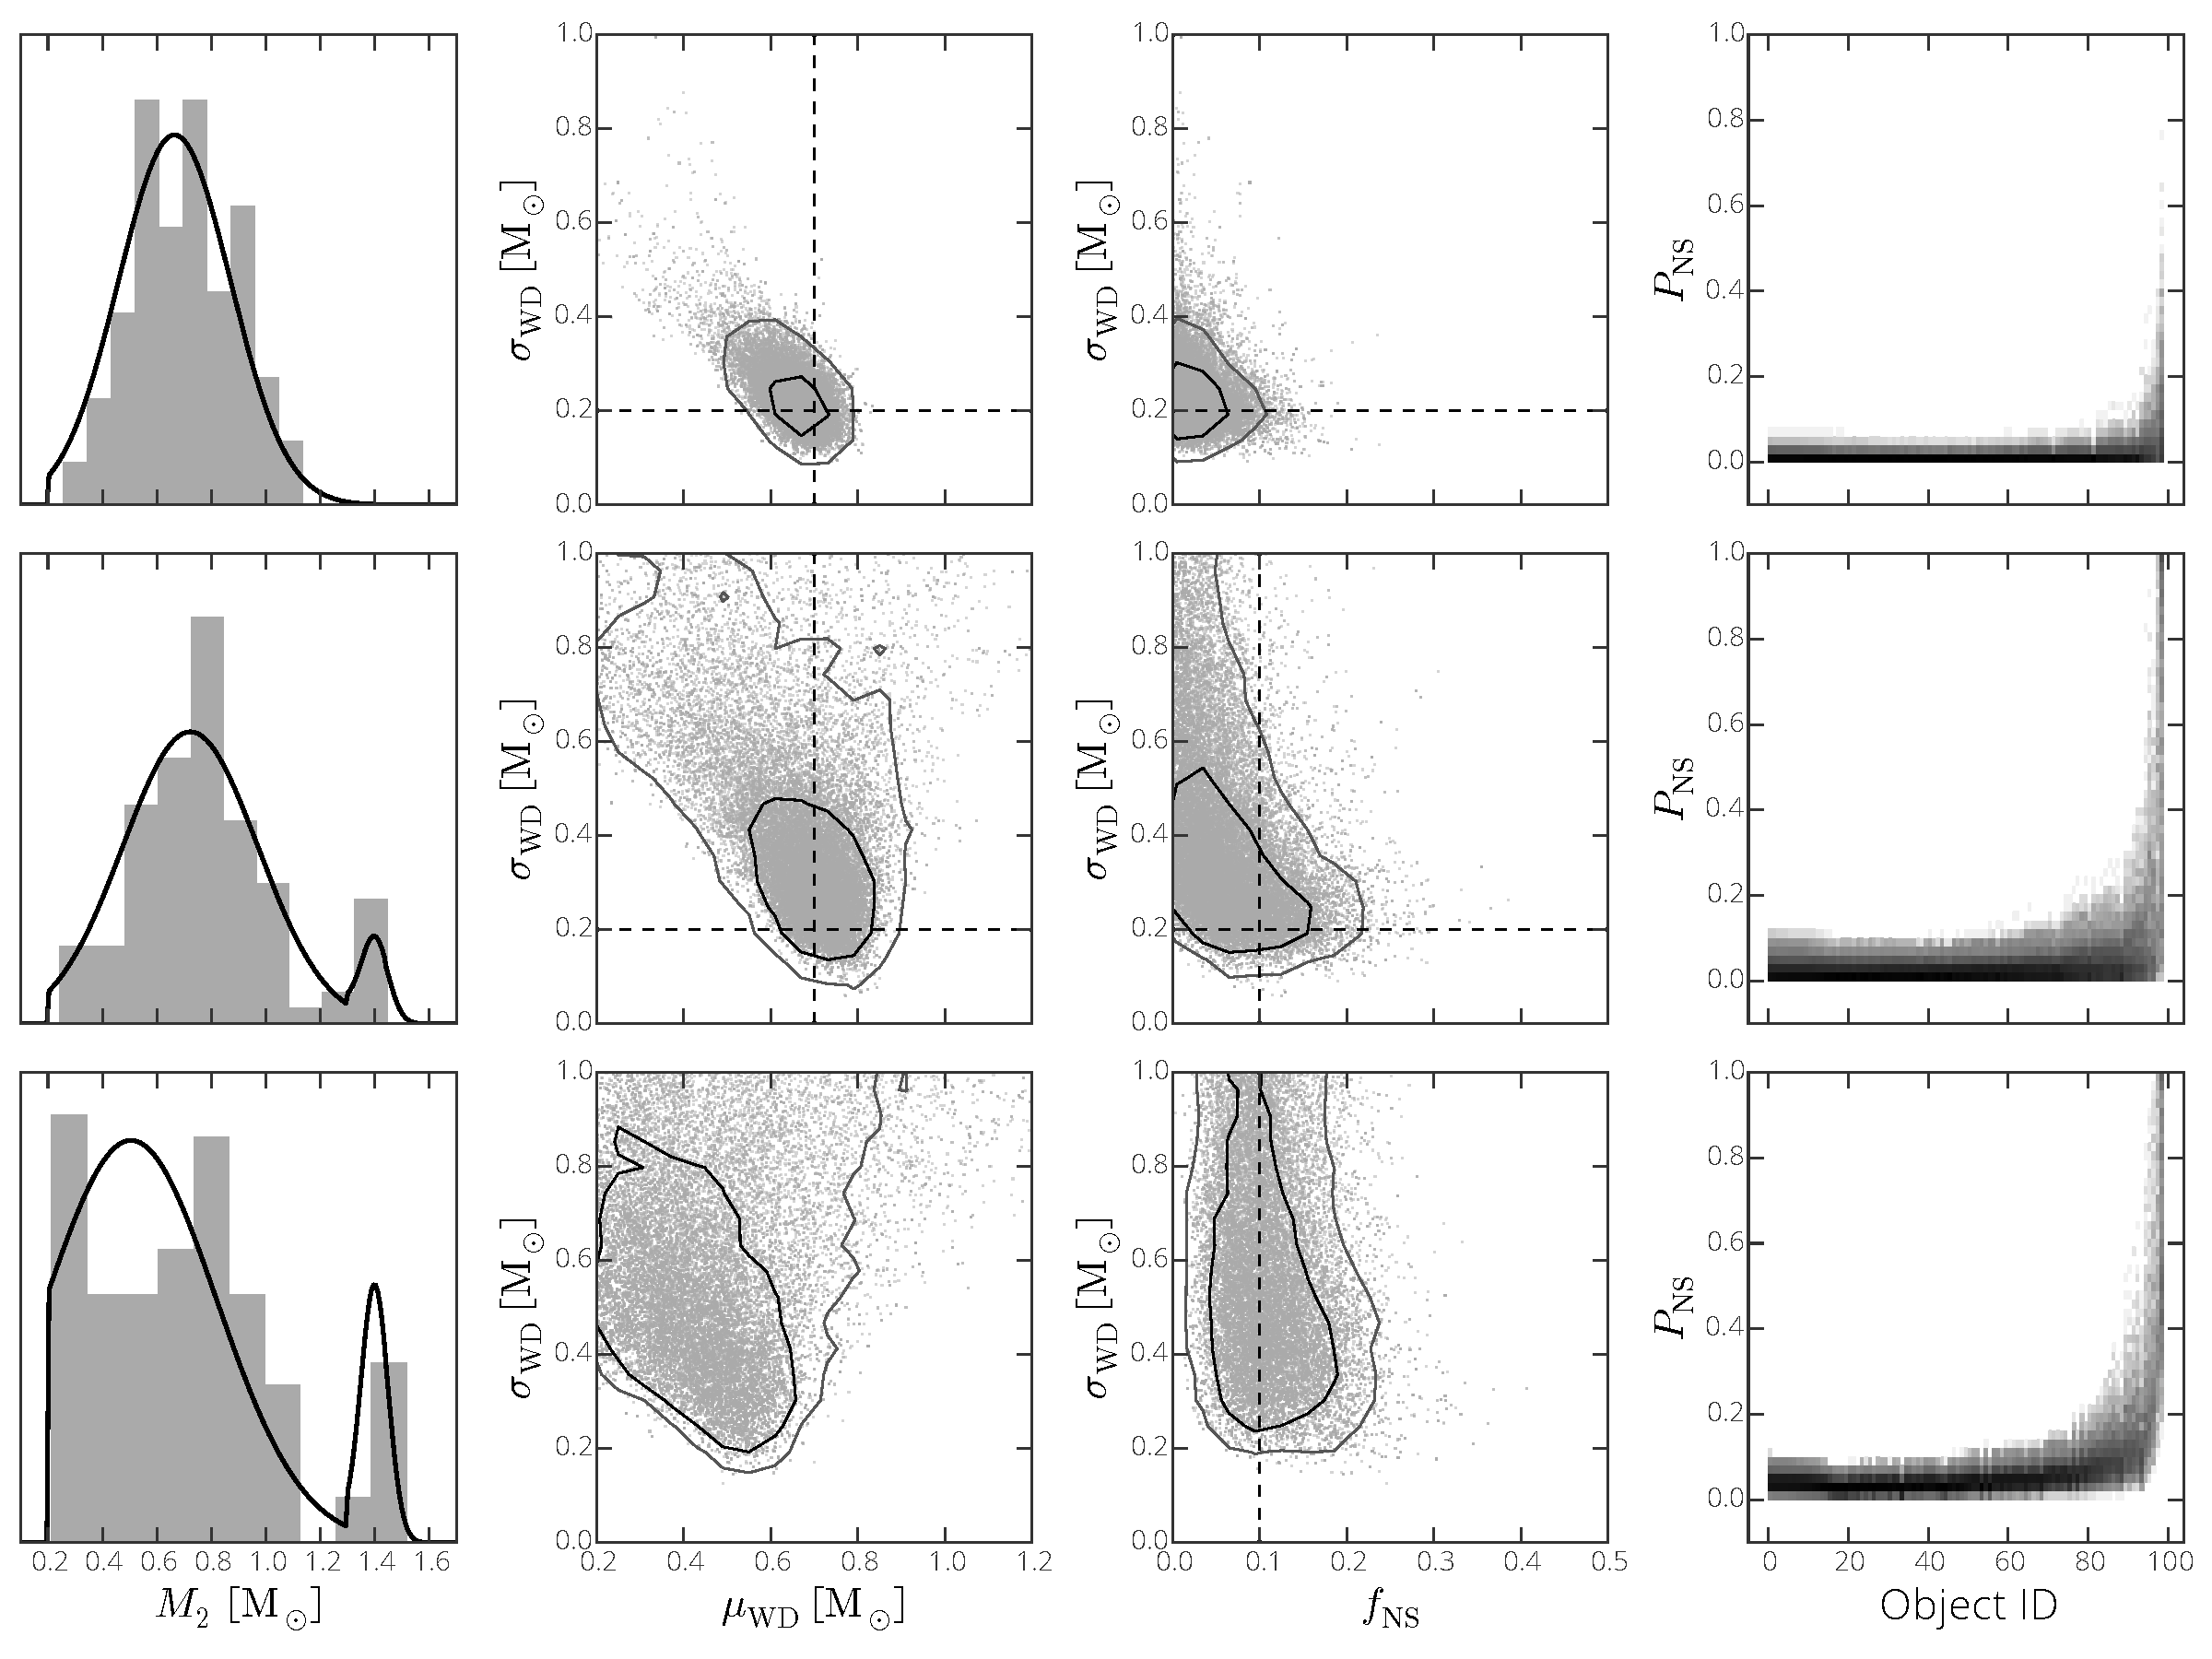
\includegraphics[width=0.95\textwidth]{many-panel.pdf}
\caption{Results from the three tests described in Section~\ref{sec:tests}. The left-most column shows histograms of $M_2$ drawn from each of our test distributions. Overplotted as solid lines are the MAP models. The second column shows samples from the posterior distributions of $\mu_{\rm WD}$ and $\sigma_{\rm WD}$. The dashed lines in the top two panels show the true values that the sample systems were drawn from. Contours designate the 68\% and 95\% contours. Since the third model was not drawn from a Gaussian distribution, there is no true parameter set. The third panel shows posterior samples for $f_{\rm NS}$ and $\sigma_{\rm WD}$, again the dashed lines show the input values. Finally, the rightmost panels list the individual systems (ordered by increasing $\mf$) and show each of their corresponding NS probabilities. }
\label{fig:tests}
\end{center}
\end{figure*}


\subsection{Test 1: Single Gaussian (WD)} \label{sec:exp1}

As a first test, we generate $M_2$ by drawing from a single, truncated Gaussian with parameters given in Table~\ref{tbl:parameters}. This test sample contains no NSs. In the top row of Figure~\ref{fig:ELM_post}, the leftmost panel shows that the maximum a posteriori (MAP) $M_2$ distribution (black line) qualitatively matches the input distribution (grey histogram). The second panel shows samples from the posterior distribution and contours that contain 68\% and 95\% of the samples. The input values lie cleanly within the inner contour in both projections of the posterior shown; the model preference toward higher masses and smaller standard deviations is due to statistical noise from our randomly generated mass distribution. The third panel shows that although the posterior $f_{\rm NS}$ distribution is consistent with 0\%, there is a tail up to $\sim$10\%. 
%Nevertheless, our model recovers the input parameters for the white dwarf companion population. 
For any set of model parameters, Equation~\ref{eq:P_NS} gives the probability of an individual system hosting a NS. using samples from our posteriors, we can determine the distribution of $P_{\rm NS}$ for each system. The fourth panel lists individual systems, ordered by $\mf$, and shows the distributions of $P_{\rm NS}$ for each. Most systems have their entire distribution of $P_{\rm NS}$ values less than $\sim$5\%.



\subsection{Test 2: Two Gaussians (WD + NS)} \label{sec:exp2}
For our next test, we use the same Gaussian distribution to generate companion masses for the WD component as the previous example, but we add an additional NS component with $f_{\rm NS} = 10\%$ and parameters described in Section~\ref{sec:experiments}. The middle row of Figure~\ref{fig:ELM_post} shows that our model again recovers the input values for $\mu_{\rm WD}$ and $\sigma_{\rm WD}$. As in Test 1, the model preference for higher $\mu_{\rm WD}$ and lower $\sigma_{\rm WD}$ is due to our randomly generated mass distribution. Importantly, the third panel shows that it also recovers $f_{\rm NS}$, however the posterior shows a substantial tail toward higher probabilities. The fourth panel indicates that some systems have near unity $P_{\rm NS}$ values; our model correctly identifies these as true NSs. However this accounts for less than half of the systems with NSs in the simulated sample; the other half have low $\mf$'s due to low inclination angles. Such systems are impossible to statistically differentiate them from those with WD companions. 




\subsection{Test 3: Uniform (WD) + Gaussian (NS)} \label{sec:exp3}
As a final test, we generate companion masses for the WD component by sampling from a uniform distribution over the range $(0.2,1.2)~\Msun$ while keeping $f_{\rm NS}=$10\%. The bottom row of Figure~\ref{fig:ELM_post} shows the results of this test. The posterior distribution in the second panel shows that the model does not converge on any one solution for $\mu_{\rm WD}$ and $\sigma_{\rm WD}$. The preference toward larger $\sigma_{\rm WD}$ is expected as it flattens the distribution to match it with the input uniform distribution. The third panel shows that the posterior distribution is spread out in $\sigma_{\rm WD}$. Interestingly, despite having a non-Gaussian input distribution for $M_2$, our model still recovers $f_{\rm NS}$ approximately as accurately as in Test 2. The fourth panel again shows that, compared to Test 2, our model is not as effective at identifying which LMWDs host NS companions.



\subsection{The ELM Sample}


The ELM WD Survey is based on the Hypervelocity Star Survey described in \citet{brown06} \citep[it also includes previously identified LMWDs in SDSS; ][]{eisenstein06,liebert04}. Objects are identified for spectroscopic follow-up by their $u-g$ versus $g-r$ colors. Since the survey is designed to find low surface gravity WDs by color, the detection probability is independent of both the mass and nature of the companion. Therefore, at least with regard to the inclination angle and companion mass, the population is unbiased.


The ELM WD sample is composed of 55 systems with radial velocity variations fit to orbital solutions, which provide precise measurements of $\period$ and $K$. Fitting the sample's high S/N spectra to templates provides precisely determine $M_1$ values. We use the spectroscopic solutions found in \citet{gianninas14}. Three systems are eclipsing binaries, with known companion masses (NLTT 11748: $M_2=0.72~\Msun$ \citep{kaplan14}, SDSS J065133.3$+$284423.3: $M_2=0.50~\Msun$ \citep{brown11b}, and SDSS J075141.2$-$014120.9: $M_2=0.97~\Msun$ \citep{kilic14}). For these systems, the likelihood reduces to:
\begin{equation}
p(\mf \given \theta) = (1-f_{\rm NS}) \mathcal{N}(M_2^* \given \mu_{\rm WD}, \sigma^2_{\rm WD})
\end{equation}
where $M_2^*$ is the mass of the WD companion in these three systems. 


The other six systems in the ELM WD sample show no evidence of orbital motion, with radial velocity upper limits of $\approx$20-50 km s$^{-1}$. Some of these systems may be in low inclination angle binaries with radial velocities below the detection limit or have orbital periods near 24 hours, which are difficult to detect \citep{ELMV}. These LMWDs could also have companions at systematically longer orbital periods resulting in orbital velocities below the detection limit. We do not include these systems in our analysis.



\begin{figure*}[h!]
\begin{center}
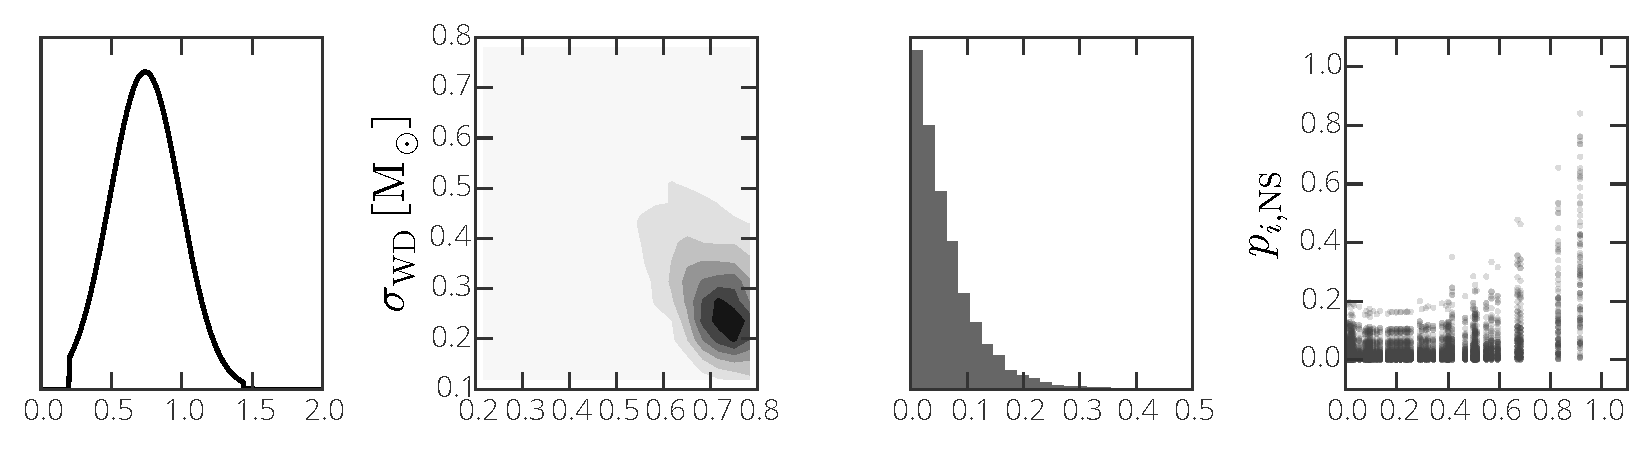
\includegraphics[width=0.95\textwidth]{real-data.pdf}
\caption{Results from applying our model to the ELM WDs. The first panel shows the MAP $M_2$ distribution (solid black) and random samples from the posterior (grey lines). The second panel shows posterior samples of $\mu$ and $\sigma$; the MAP Gaussian model has $\mu_{\rm WD}= 0.71~\Msun$ and $\sigma_{\rm WD}= 0.26~\Msun$. The third panel shows posterior samples of $\mu$ and $f_{\rm NS}$. The last panel lists individual LMWDs in the ELM sample (ordered by increasing $\mf$) and shows each of their corresponding NS probabilities. The three systems with all $P_{\rm NS}$ values at 0\% are the three eclipsing systems with measured $M_2$.}
\label{fig:ELM_post}
\end{center}
\end{figure*}



\section{Results and Discussion}

The results from applying our model to the ELM sample are shown in Figure \ref{fig:ELM_post}. The MAP model has parameters $\mu_{\rm WD} = 0.71~\Msun$, $\sigma_{\rm WD} = 0.26~\Msun$, and $f_{\rm NS} = 0\%$. The marginal posterior over $\mu_{\rm WD}$ and $\sigma_{\rm WD}$ has a tail towards larger variances, which could indicate that the true WD distribution is not exactly Gaussian. It is interesting that the best fit Gaussian for the companions to the ELM WD sample is similar to that of the population of single DA WDs in SDSS with a mean of 0.6 $\Msun$ \citep{kleinman13}. Our distribution is significantly wider ({\bf $\sigma \approx 0.26~\Msun$} compared with $\sigma \approx 0.1~\Msun$), possibly due to mass transfer affecting the mass distribution of the unseen primary WDs as well.


Our results are independent of astrophysical expectations since they do not include any priors on $\mu_{\rm WD}$ and $\sigma_{\rm WD}$, apart from limits for $M_2$ of 0.2 \Msun\,(based on observations of LMWDs) and \wdupper~\Msun\,(based on the Chandrasekhar mass). In principle, priors could be added based on population synthesis models that suggest that there are two dominant companion populations to LMWDs, composed of CO and He core WDs \citep{han98}. The ratio and distribution of these two populations depends on the exact stellar evolution prescriptions assumed \citep[see discussion in, e.g., ][]{toonen12}. Our results here suggest the companion sample is composed mainly of CO WDs. Our model could be expanded to include a two Gaussian model --- one for each WD population. The ratio of these populations could potentially place an important constraint on population synthesis models. However, we have found that there is not enough data to motivate adding additional freedom to the model in the form of a second WD component.


The third panel in Figure~\ref{fig:ELM_post} shows a NS fraction strongly peaked toward 0. However, there is a significant tail toward higher NS probabilities. Our model indicates $f_{\rm NS} <16\%$ at the 68\% confidence level, in agreement with independent constraints from \citet{vLeeuwen07} ($f_{\rm NS}<18\pm5$\%), based on the non-detection of radio emission from eight LMWD targets, and from \citet{agueros09b} ($f_{\rm NS}<10\substack{+4 \\ -2}~\%$), based on non-detections of radio emission from an expanded sample of 15 LMWD targets in the ELM WD sample. Because it may be radio quiet or beamed away from us, a NS companion to these LMWDs may not be detectable \citep{vLeeuwen07}. All NSs give off blackbody radiation peaked in X-ray wavelengths, so X-ray follow-up provides a more stringent test on the potential for a NS companion \citep{agueros09a}. Previous searches for LMWDs with X-ray counterparts have all been non-detections \citep{ELMII,ELMIV,kilic13,kilic14}. However, we show here that all of those sources have a low probability of hosting a NS companion. If the two systems with the highest $P_{\rm NS}$, SDSS J081133.6$+$022556.8 and SDSS J174140.5$+$652638.7, also lack X-ray counterparts, then even more stringent constraints can be placed on $f_{\rm NS}$. 

It is worth noting that systems with NS companions cannot necessarily be differentiated from those with WD companions through the mass function and LMWD mass alone. Therefore there is a non-negligible probability that {\it any} LMWD could host a NS companion. 

%These systems are ideal candidates for radio and X-ray searches for NS companions. 
%Radio observations of these objects are in progress, however 


%It is worth noting that the fourth panels in our test cases in Figure~\ref{fig:tests} shows that our model is fairly good at identifying those systems most likely to host NS's. However it also shows that roughly half of the LMWDs with NS companions may appear with a deceptively low $f_{\rm NS}$ due to the inclination angle. 

To determine the probability of any particular LMWD of hosting a NS, we make our model posteriors publicly available on fig{\bf share}.\footnote{\url{http://dx.doi.org/10.6084/m9.figshare.1206621}} We further provide a {\tt python} script that calculates $P_{\rm NS}$ and the mass distribution for a WD companion for any LMWD with a measured $M_1$ and $\mf$. This script can be applied to newly discovered LMWDs as well as those already in the ELM sample.



\section{Conclusions}

We have developed a statistical model to infer the companion mass distribution for a sample of single-lined, spectroscopic binaries. This model can be applied to any such sample with measured $M_1$. When applied to three separate test cases with WD and NS companion masses drawn from different distributions, our model recovers the correct input parameters; even if the companion mass distribution is not drawn from a Gaussian distribution, our model still infers the input NS fraction within a few percent.


We then applied our model to the set of WDs from the ELM WD survey. Our model indicates that the fraction of ELM WDs with NS companions is consistent with 0\%, but could be up to $\sim$16\% (within 1-$\sigma$). We identify SDSS J081133.6$+$022556.8 and SDSS J174140.5$+$652638.7 as having the highest probabilities of hosting a NS companion and suggest that X-ray and radio follow-up is warranted. Our model further suggests that the majority of ELM WDs have CO-core WD companions. This is in contrast to predictions from population synthesis models which predict the dominant companion population should be He-core WDs \citep{toonen12}. 

%In particular, we plan to develop our method to quantitatively compare our model to the results of population synthesis codes, potentially constraining the formation of LMWDs.

There are several ways in which this model can be expanded. Recently, \citet{hermes14} made high-speed photometric observations of 20 LMWDs in the ELM sample. Based on non-detection of eclipses and modeling of photometric variability, these authors set limits on the inclination angles of these systems, which could be included in our model. Furthermore, tighter constraints can be placed on $f_{\rm NS}$ by including radio and X-ray non-detection data. Finally, we plan to develop our method to quantitatively compare our model to the results of population synthesis codes, potentially constraining the formation of LMWDs.

%Our model is applicable to any arbitrary set of single-lined spectroscopic binaries. Applying this method to various populations can help to constrain the formation of particularly classes of binaries. 



\acknowledgements
The authors wish to acknowledge David Hogg and DJ D'Orazio for useful discussions, and the organizers of the \emph{AstroData Hack Week} (2014). 
APW is supported by a National Science Foundation Graduate Research Fellowship under Grant No.\ 11-44155. 
This research made use of Astropy, a community-developed core \texttt{Python} package for Astronomy \citep{astropy13}. \\

\bibliographystyle{apj}



\begin{thebibliography}{36}
\expandafter\ifx\csname natexlab\endcsname\relax\def\natexlab#1{#1}\fi

\bibitem[{{Ag{\"u}eros} {et~al.}(2009{\natexlab{a}}){Ag{\"u}eros}, {Camilo},
  {Silvestri}, {Kleinman}, {Anderson}, \& {Liebert}}]{agueros09b}
{Ag{\"u}eros}, M.~A., {Camilo}, F., {Silvestri}, N.~M., {Kleinman}, S.~J.,
  {Anderson}, S.~F., \& {Liebert}, J.~W. 2009{\natexlab{a}}, \apj, 697, 283

\bibitem[{{Ag{\"u}eros} {et~al.}(2009{\natexlab{b}}){Ag{\"u}eros}, {Heinke},
  {Camilo}, {Kilic}, {Anderson}, {Freire}, {Kleinman}, {Liebert}, \&
  {Silvestri}}]{agueros09a}
{Ag{\"u}eros}, M.~A. {et~al.} 2009{\natexlab{b}}, \apjl, 700, L123

\bibitem[{{Antoniadis} {et~al.}(2012){Antoniadis}, {van Kerkwijk}, {Koester},
  {Freire}, {Wex}, {Tauris}, {Kramer}, \& {Bassa}}]{antoniadis12}
{Antoniadis}, J., {van Kerkwijk}, M.~H., {Koester}, D., {Freire}, P.~C.~C.,
  {Wex}, N., {Tauris}, T.~M., {Kramer}, M., \& {Bassa}, C.~G. 2012, \mnras,
  423, 3316

\bibitem[{{Astropy Collaboration} {et~al.}(2013){Astropy Collaboration},
  {Robitaille}, {Tollerud}, {Greenfield}, {Droettboom}, {Bray}, {Aldcroft},
  {Davis}, {Ginsburg}, {Price-Whelan}, {Kerzendorf}, {Conley}, {Crighton},
  {Barbary}, {Muna}, {Ferguson}, {Grollier}, {Parikh}, {Nair}, {Unther},
  {Deil}, {Woillez}, {Conseil}, {Kramer}, {Turner}, {Singer}, {Fox}, {Weaver},
  {Zabalza}, {Edwards}, {Azalee Bostroem}, {Burke}, {Casey}, {Crawford},
  {Dencheva}, {Ely}, {Jenness}, {Labrie}, {Lim}, {Pierfederici}, {Pontzen},
  {Ptak}, {Refsdal}, {Servillat}, \& {Streicher}}]{astropy13}
{Astropy Collaboration} {et~al.} 2013, \aap, 558, A33

\bibitem[{{Bassa} {et~al.}(2006){Bassa}, {van Kerkwijk}, {Koester}, \&
  {Verbunt}}]{bassa06}
{Bassa}, C.~G., {van Kerkwijk}, M.~H., {Koester}, D., \& {Verbunt}, F. 2006,
  \aap, 456, 295

\bibitem[{{Benvenuto} \& {De Vito}(2005)}]{benvenuto05}
{Benvenuto}, O.~G., \& {De Vito}, M.~A. 2005, \mnras, 362, 891

\bibitem[{{Brown} {et~al.}(2013){Brown}, {Kilic}, {Allende Prieto},
  {Gianninas}, \& {Kenyon}}]{ELMV}
{Brown}, W.~R., {Kilic}, M., {Allende Prieto}, C., {Gianninas}, A., \&
  {Kenyon}, S.~J. 2013, \apj, 769, 66

\bibitem[{{Brown} {et~al.}(2010){Brown}, {Kilic}, {Allende Prieto}, \&
  {Kenyon}}]{ELMI}
{Brown}, W.~R., {Kilic}, M., {Allende Prieto}, C., \& {Kenyon}, S.~J. 2010,
  \apj, 723, 1072

\bibitem[{{Brown} {et~al.}(2012){Brown}, {Kilic}, {Allende Prieto}, \&
  {Kenyon}}]{ELMIII}
---. 2012, \apj, 744, 142

\bibitem[{{Brown} {et~al.}(2011){Brown}, {Kilic}, {Hermes}, {Allende Prieto},
  {Kenyon}, \& {Winget}}]{brown11b}
{Brown}, W.~R., {Kilic}, M., {Hermes}, J.~J., {Allende Prieto}, C., {Kenyon},
  S.~J., \& {Winget}, D.~E. 2011, \apjl, 737, L23

\bibitem[{{Callanan} {et~al.}(1998){Callanan}, {Garnavich}, \&
  {Koester}}]{callanan98}
{Callanan}, P.~J., {Garnavich}, P.~M., \& {Koester}, D. 1998, \mnras, 298, 207

\bibitem[{{Foreman-Mackey} {et~al.}(2013){Foreman-Mackey}, {Hogg}, {Lang}, \&
  {Goodman}}]{foremanmackey13}
{Foreman-Mackey}, D., {Hogg}, D.~W., {Lang}, D., \& {Goodman}, J. 2013, \pasp,
  125, 306

\bibitem[{{Gianninas} {et~al.}(2014){Gianninas}, {Dufour}, {Kilic}, {Brown},
  {Bergeron}, \& {Hermes}}]{gianninas14}
{Gianninas}, A., {Dufour}, P., {Kilic}, M., {Brown}, W.~R., {Bergeron}, P., \&
  {Hermes}, J.~J. 2014, \apj, 794, 35

\bibitem[Goodman~\&\ Weare(2010)]{goodman10}
Goodman,~J. \& Weare,\ J.,
2010, Comm.\ App.\ Math.\ Comp.\ Sci., 5, 65

\bibitem[{{Han}(1998)}]{han98}
{Han}, Z. 1998, \mnras, 296, 1019

\bibitem[{{Hermes} {et~al.}(2014){Hermes}, {Brown}, {Kilic}, {Gianninas},
  {Chote}, {Sullivan}, {Winget}, {Bell}, {Falcon}, {Winget}, {Mason},
  {Harrold}, \& {Montgomery}}]{hermes14}
{Hermes}, J.~J. {et~al.} 2014, \apj, 792, 39

\bibitem[{{Jia} \& {Li}(2014)}]{jia14}
{Jia}, K., \& {Li}, X.-D. 2014, \apj, 791, 127

\bibitem[{{Kaplan} {et~al.}(2014){Kaplan}, {Marsh}, {Walker}, {Bildsten},
  {Bours}, {Breedt}, {Copperwheat}, {Dhillon}, {Howell}, {Littlefair},
  {Shporer}, \& {Steinfadt}}]{kaplan14}
{Kaplan}, D.~L. {et~al.} 2014, \apj, 780, 167

\bibitem[{{Kilic} {et~al.}(2011){Kilic}, {Brown}, {Allende Prieto},
  {Ag{\"u}eros}, {Heinke}, \& {Kenyon}}]{ELMII}
{Kilic}, M., {Brown}, W.~R., {Allende Prieto}, C., {Ag{\"u}eros}, M.~A.,
  {Heinke}, C., \& {Kenyon}, S.~J. 2011, \apj, 727, 3

\bibitem[{{Kilic} {et~al.}(2012){Kilic}, {Brown}, {Allende Prieto}, {Kenyon},
  {Heinke}, {Ag{\"u}eros}, \& {Kleinman}}]{ELMIV}
{Kilic}, M., {Brown}, W.~R., {Allende Prieto}, C., {Kenyon}, S.~J., {Heinke},
  C.~O., {Ag{\"u}eros}, M.~A., \& {Kleinman}, S.~J. 2012, \apj, 751, 141

\bibitem[{{Kilic} {et~al.}(2013){Kilic}, {Gianninas}, {Brown}, {Harris},
  {Dahn}, {Ag{\"u}eros}, {Heinke}, {Kenyon}, {Panei}, \& {Camilo}}]{kilic13}
{Kilic}, M. {et~al.} 2013, \mnras, 434, 3582

\bibitem[{{Kilic} {et~al.}(2014){Kilic}, {Hermes}, {Gianninas}, {Brown},
  {Heinke}, {Ag{\"u}eros}, {Chote}, {Sullivan}, {Bell}, \& {Harrold}}]{kilic14}
---. 2014, \mnras, 438, L26

\bibitem[{{Kilic} {et~al.}(2007){Kilic}, {Stanek}, \& {Pinsonneault}}]{kilic07}
{Kilic}, M., {Stanek}, K.~Z., \& {Pinsonneault}, M.~H. 2007, \apj, 671, 761

\bibitem[{{Kiziltan} {et~al.}(2013){Kiziltan}, {Kottas}, {De Yoreo}, \&
  {Thorsett}}]{kiziltan13}
{Kiziltan}, B., {Kottas}, A., {De Yoreo}, M., \& {Thorsett}, S.~E. 2013, \apj,
  778, 66

\bibitem[{{Kleinman} {et~al.}(2013){Kleinman}, {Kepler}, {Koester}, {Pelisoli},
  {Pe{\c c}anha}, {Nitta}, {Costa}, {Krzesinski}, {Dufour}, {Lachapelle},
  {Bergeron}, {Yip}, {Harris}, {Eisenstein}, {Althaus}, \&
  {C{\'o}rsico}}]{kleinman13}
{Kleinman}, S.~J. {et~al.} 2013, \apjs, 204, 5

\bibitem[{{Liebert} {et~al.}(2005){Liebert}, {Bergeron}, \&
  {Holberg}}]{liebert05}
{Liebert}, J., {Bergeron}, P., \& {Holberg}, J.~B. 2005, \apjs, 156, 47

\bibitem[{{Marsh} {et~al.}(1995){Marsh}, {Dhillon}, \& {Duck}}]{marsh95}
{Marsh}, T.~R., {Dhillon}, V.~S., \& {Duck}, S.~R. 1995, \mnras, 275, 828

\bibitem[{{Nelemans} {et~al.}(2000){Nelemans}, {Verbunt}, {Yungelson}, \&
  {Portegies Zwart}}]{nelemans00}
{Nelemans}, G., {Verbunt}, F., {Yungelson}, L.~R., \& {Portegies Zwart}, S.~F.
  2000, \aap, 360, 1011

\bibitem[{{Nelemans} {et~al.}(2001){Nelemans}, {Yungelson}, {Portegies Zwart},
  \& {Verbunt}}]{nelemans01}
{Nelemans}, G., {Yungelson}, L.~R., {Portegies Zwart}, S.~F., \& {Verbunt}, F.
  2001, \aap, 365, 491

\bibitem[{{{\"O}zel} {et~al.}(2012){{\"O}zel}, {Psaltis}, {Narayan}, \& {Santos
  Villarreal}}]{ozel12}
{{\"O}zel}, F., {Psaltis}, D., {Narayan}, R., \& {Santos Villarreal}, A. 2012,
  \apj, 757, 55

\bibitem[{{Smedley} {et~al.}(2014){Smedley}, {Tout}, {Ferrario}, \&
  {Wickramasinghe}}]{smedley14}
{Smedley}, S.~L., {Tout}, C.~A., {Ferrario}, L., \& {Wickramasinghe}, D.~T.
  2014, \mnras, 437, 2217

\bibitem[{{Toonen} {et~al.}(2012){Toonen}, {Nelemans}, \& {Portegies
  Zwart}}]{toonen12}
{Toonen}, S., {Nelemans}, G., \& {Portegies Zwart}, S. 2012, \aap, 546, A70

\bibitem[{{van der Sluys} {et~al.}(2006){van der Sluys}, {Verbunt}, \&
  {Pols}}]{vdSluys06}
{van der Sluys}, M.~V., {Verbunt}, F., \& {Pols}, O.~R. 2006, \aap, 460, 209

\bibitem[{{van Kerkwijk} {et~al.}(1996){van Kerkwijk}, {Bergeron}, \&
  {Kulkarni}}]{vKerkwijk96}
{van Kerkwijk}, M.~H., {Bergeron}, P., \& {Kulkarni}, S.~R. 1996, \apjl, 467,
  L89

\bibitem[{{van Leeuwen} {et~al.}(2007){van Leeuwen}, {Ferdman}, {Meyer}, \&
  {Stairs}}]{vLeeuwen07}
{van Leeuwen}, J., {Ferdman}, R.~D., {Meyer}, S., \& {Stairs}, I. 2007, \mnras,
  374, 1437

\bibitem[{{Woods} {et~al.}(2012){Woods}, {Ivanova}, {van der Sluys}, \&
  {Chaichenets}}]{woods12}
{Woods}, T.~E., {Ivanova}, N., {van der Sluys}, M.~V., \& {Chaichenets}, S.
  2012, \apj, 744, 12

\end{thebibliography}


%\bibliography{refs}
  



\end{document}

